% Data: completed presentation/CG1_PRIMARY_COMPARISONS.csv.
% Signs of cg1_minus_baseline_detections across each comparator's 32 strata.
\begin{figure}[t]
\centering
\begingroup
\definecolor{resultblue}{HTML}{0072B2}
\definecolor{resultorange}{HTML}{D55E00}
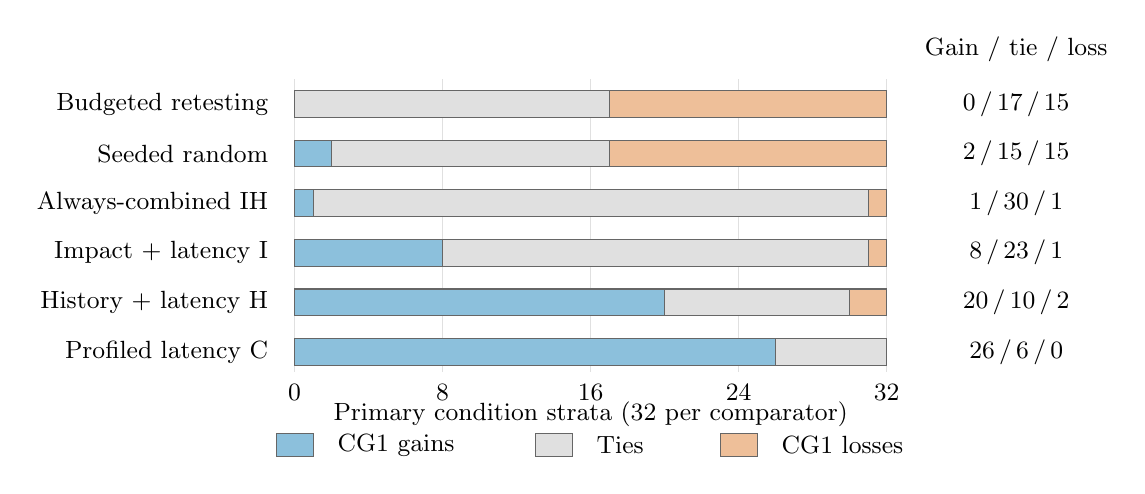
\begin{tikzpicture}[x=0.235cm,y=0.63cm,font=\small]
  \foreach \tick in {0,8,16,24,32} {
    \draw[black!12] (\tick,-0.4) -- (\tick,5.5);
    \node[below] at (\tick,-0.45) {\tick};
  }
  \node at (39,6.1) {Gain / tie / loss};
  % Comparator, row, CG1 gains, detection ties, CG1 losses.
  \foreach \method/\row/\gain/\tie/\loss in {
    {Budgeted retesting}/5/0/17/15,
    {Seeded random}/4/2/15/15,
    {Always-combined IH}/3/1/30/1,
    {Impact + latency I}/2/8/23/1,
    {History + latency H}/1/20/10/2,
    {Profiled latency C}/0/26/6/0} {
    \node[anchor=east] at (-0.9,\row) {\method};
    \pgfmathtruncatemacro{\tiebound}{\gain+\tie}
    \ifnum\gain>0
      \filldraw[fill=resultblue!45,draw=black!60]
        (0,{\row-0.27}) rectangle (\gain,{\row+0.27});
    \fi
    \filldraw[fill=black!12,draw=black!60]
      (\gain,{\row-0.27}) rectangle (\tiebound,{\row+0.27});
    \ifnum\loss>0
      \filldraw[fill=resultorange!40,draw=black!60]
        (\tiebound,{\row-0.27}) rectangle (32,{\row+0.27});
    \fi
    \node at (39,\row) {\gain\,/\,\tie\,/\,\loss};
  }
  \node at (16,-1.25) {Primary condition strata (32 per comparator)};
  \filldraw[fill=resultblue!45,draw=black!60] (-1,-2.1) rectangle (1,-1.65);
  \node[anchor=west] at (1.8,-1.88) {CG1 gains};
  \filldraw[fill=black!12,draw=black!60] (13,-2.1) rectangle (15,-1.65);
  \node[anchor=west] at (15.8,-1.88) {Ties};
  \filldraw[fill=resultorange!40,draw=black!60] (23,-2.1) rectangle (25,-1.65);
  \node[anchor=west] at (25.8,-1.88) {CG1 losses};
\end{tikzpicture}
\endgroup
\caption{CG1 detection comparisons across all 32 primary strata. Bars and
printed triples count gains, ties and losses against each comparator. CG1 has
no detection gain against budgeted catalog retesting, fifteen losses against both
budgeted retesting and seeded random, and one gain and one loss against
always-combined. These are counts of finite experimental strata, each
aggregating three recorded passes, rather than independent bugs or population
effect estimates. Detection ties do not imply equal requests, equal discordant
alarms or Pareto equivalence.}
\Description{Six stacked bars show CG1 detection gain, tie and loss counts out
of 32 primary strata. Against budgeted catalog retesting the counts are 0, 17 and 15;
seeded random 2, 15 and 15; always-combined IH 1, 30 and 1; impact plus
latency I 8, 23 and 1; history plus latency H 20, 10 and 2; profiled latency C
26, 6 and 0. Numeric triples provide the same information without color.}
\label{fig:result-comparators}
\end{figure}
